\chapter{Página Web}
    
    \section{Introducción}
    
        La página web desarrollada para \textcolor{dark_violet}{\textbf{GraviCap}} juega un papel fundamental en la difusión y comunicación del proyecto. Su creación responde a la necesidad de tener una plataforma en línea donde se pueda acceder fácilmente a toda la información relevante sobre el proyecto, sus objetivos, sus integrantes y las fases de desarrollo. Este sitio web no solo sirve como un medio de promoción, sino que también actúa como un canal interactivo entre el equipo y el público interesado.\par
        A lo largo del desarrollo del proyecto, consideramos esencial contar con una herramienta que fuera accesible para cualquier persona interesada en conocer más sobre \textcolor{dark_violet}{\textbf{GraviCap}}. Por ello, el sitio web se construyó con un diseño intuitivo y funcional, con el objetivo de proporcionar información clara y precisa, así como facilitar la interacción directa con los visitantes a través de un formulario de contacto. Asimismo, la página está pensada para ser compatible con dispositivos móviles y de escritorio, asegurando que cualquier usuario pueda acceder a la información sin inconvenientes, independientemente del dispositivo que utilice.\par
        Este capítulo describe en detalle el propósito de la página web, su estructura técnica, los componentes que la componen y el proceso seguido para su implementación. Desde la creación de los componentes en Vue.js hasta su despliegue final utilizando Vercel.app, se documentan los pasos clave y las decisiones técnicas que permitieron la construcción de un sitio web eficiente y profesional para el proyecto \textcolor{dark_violet}{\textbf{GraviCap}}.\par

    \section{Función}
        El objetivo principal de la página web es proporcionar una plataforma accesible para que los usuarios interesados en el proyecto \textcolor{dark_violet}{\textbf{GraviCap}} puedan obtener más información sobre el mismo, conocer a los integrantes del equipo y entender el proceso que llevó al desarrollo del proyecto desde su concepción hasta la implementación final. Además, la página web ofrece la posibilidad de que los usuarios se pongan en contacto con nosotros a través de un formulario de contacto, facilitando la comunicación directa por correo electrónico. La promoción de la página se realizará mediante un enlace compartido en la cuenta de Instagram de \textcolor{dark_violet}{\textbf{GraviCap}}, usando una herramienta de linktree, lo que asegurará su visibilidad en las redes sociales.\par
        
    \section{Estructura}
            \subsection{Componentes}
                La estructura de la página web está organizada de manera modular, dividiéndose en varios componentes que permiten la navegación sencilla entre las diferentes secciones. Estos componentes fueron desarrollados en Vue.js, lo que facilita su integración y reutilización en diferentes partes de la página. Se crearon cuatro componentes principales, cada uno con una funcionalidad específica, y un componente adicional que es común en todas las rutas de la página.\par
                
                \subsubsection{App.vue}
                    El componente App.vue se mantiene activo sin importar la ruta seleccionada dentro de la página web, sirviendo como una estructura común a todas las secciones. Este componente contiene un header con el logotipo de \textcolor{dark_violet}{GraviCap} y un texto con el nombre del proyecto, ambos actuando como enlaces que redirigen al subcomponente Home. Además, se incluyen tres opciones de navegación: Sobre Nosotros, Galería y Contáctanos, que funcionan como rutas hacia sus respectivos subcomponentes. También se han añadido iconos para redirigir a las cuentas de Instagram y GitHub del proyecto, facilitando el acceso directo a las redes sociales y al repositorio del código.\par
                    
                    \begin{figure}[!ht]
                        \centering
                        
\includegraphics[width=\linewidth]{Imagenes/Página Web/App.jpg}
                        \caption{Componente de App.vue}
                        \label{fig:pw1}
                    \end{figure}
                    
                \subsubsection{HomeView.vue}
                    El subcomponente HomeView.vue es la página principal que se carga por defecto al ingresar al sitio. Está dividida en dos partes: un grid a la izquierda que contiene el eslogan del proyecto junto con un resumen breve y claro sobre el propósito de \textcolor{dark_violet}{GraviCap}, y un grid a la derecha que presenta un título con tres subtítulos explicando los beneficios clave del proyecto. Este subcomponente proporciona al usuario una visión general inmediata de lo que trata el proyecto y sus ventajas.\par
                    
                    \begin{figure} [H]
                    \centering
                    \begin{subfigure}{0.5\textwidth}
                        \centering
                        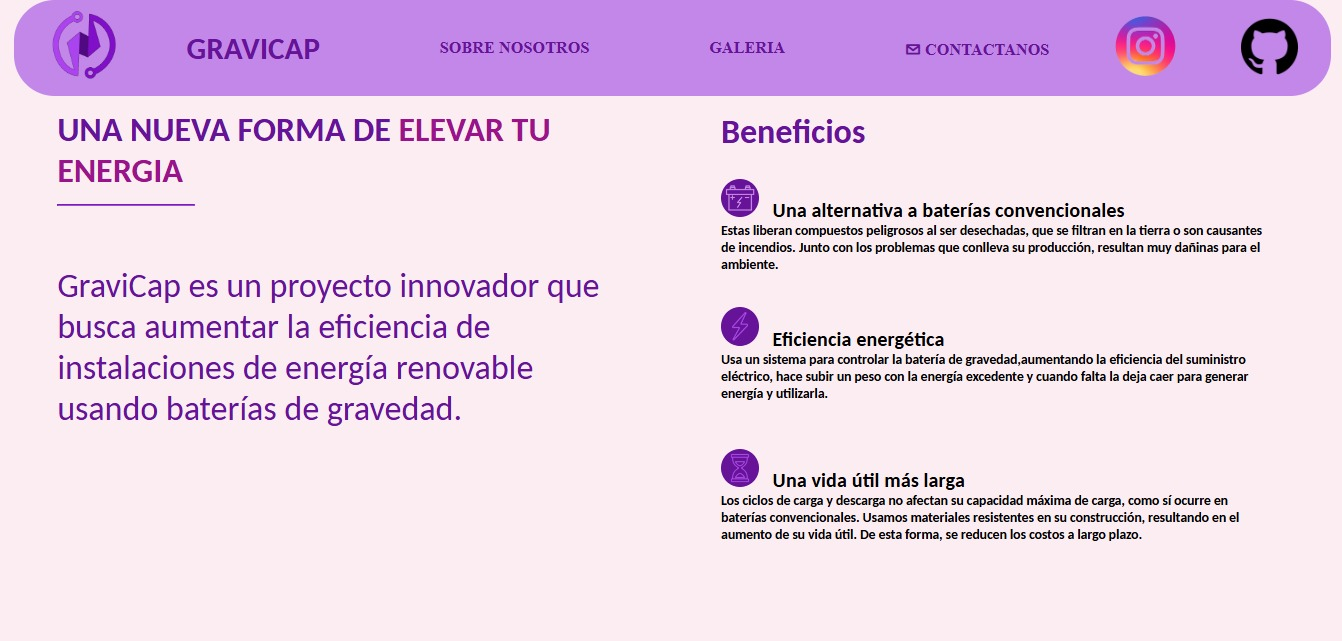
\includegraphics[width=\textwidth]{Imagenes/Página Web/Computadora/HomeScreen.jpg}
                        \caption{Computadora}
                        \label{fig:pw2.1}
                    \end{subfigure}
                    \hfill
                    \begin{subfigure}{0.4\textwidth}
                        \centering
                        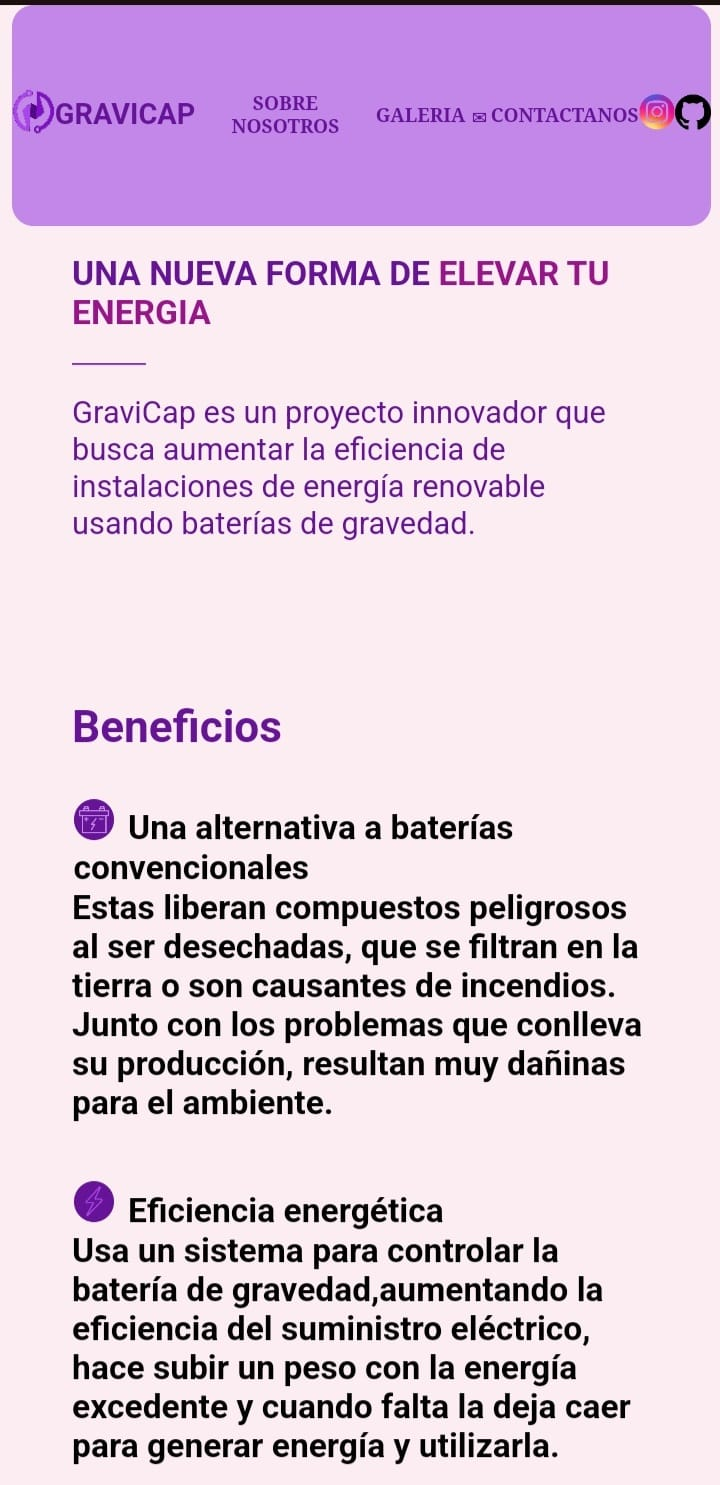
\includegraphics[width=0.5\textwidth]{Imagenes/Página Web/Celular/Homescreen.jpg}
                        \caption{Celular}
                        \label{fig:pw2.2}
                    \end{subfigure}
                    \hfill
                            
                    \caption{Componente de HomeView.vue}
                    \label{fig:pw2}
                    \end{figure}
                    
                \subsubsection{NosotrosView.vue}
                    Este subcomponente, NosotrosView.vue, está organizado en dos secciones principales. A la izquierda, el título "¿Quiénes Somos?" ofrece una explicación sobre el origen del equipo de trabajo, los objetivos del grupo y el propósito detrás de este proyecto. A la derecha, se muestra una galería de imágenes con las fotos de los integrantes del equipo, acompañadas por sus respectivos roles dentro del desarrollo del proyecto, brindando una presentación visual y detallada de quienes están detrás de \textcolor{dark_violet}{GraviCap}.\par

                    \begin{figure} [H]
                    \centering
                    \begin{subfigure}{0.5\textwidth}
                        \centering
                        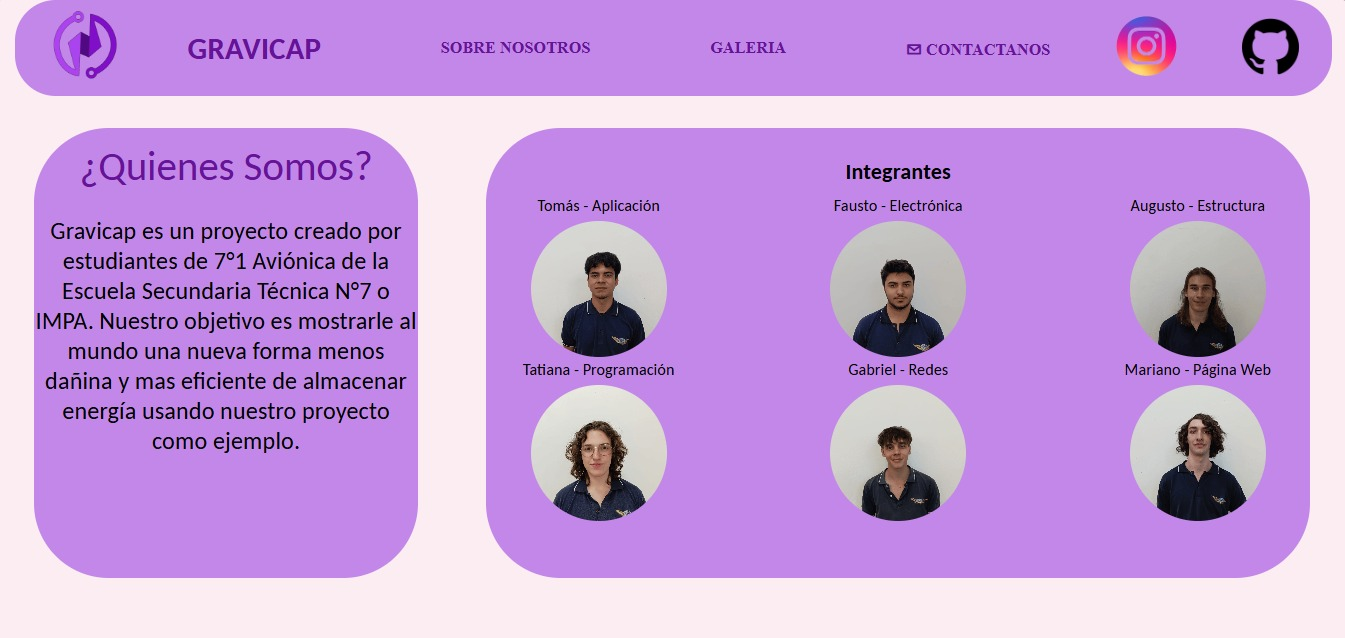
\includegraphics[width=\textwidth]{Imagenes/Página Web/Computadora/Integrantes.jpg}
                        \caption{Computadora}
                        \label{fig:pw3.1}
                    \end{subfigure}
                    \hfill
                    \begin{subfigure}{0.4\textwidth}
                        \centering
                        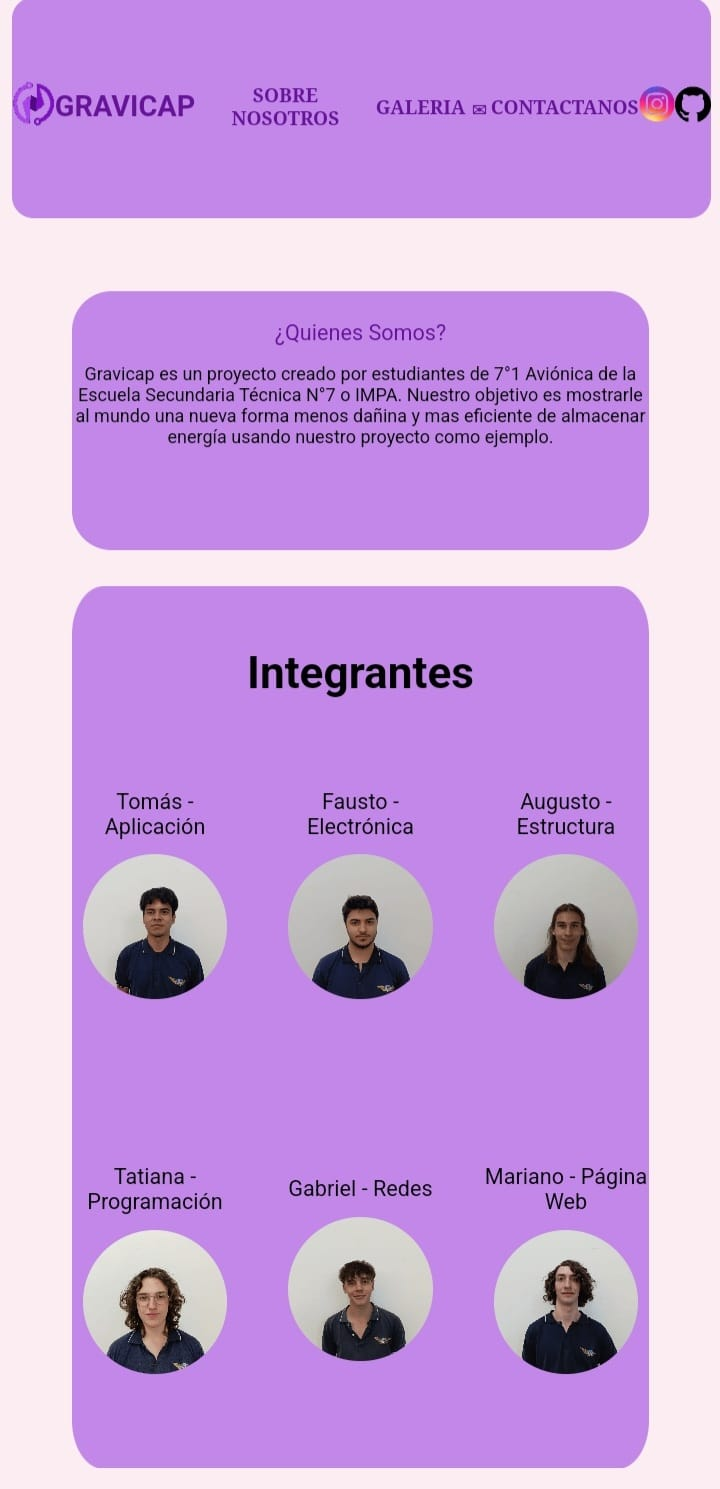
\includegraphics[width=0.5\textwidth]{Imagenes/Página Web/Celular/Integrantes.jpg}
                        \caption{Celular}
                        \label{fig:pw3.2}
                    \end{subfigure}
                    \hfill
                            
                    \caption{NosotrosView.vue}
                    \label{fig:pw3}
                    \end{figure}
                    
                \subsubsection{GaleríaView.vue}
                    El subcomponente GaleríaView.vue se encarga de mostrar las imágenes más relevantes relacionadas con el proyecto. Se organiza en un diseño de grid con múltiples columnas, donde cada imagen está acompañada de un título que explica brevemente de qué trata. Este subcomponente permite a los usuarios explorar visualmente el desarrollo y avances del proyecto a lo largo del tiempo.\par

                    \begin{figure} [H]
                    \centering
                    \begin{subfigure}{0.5\textwidth}
                        \centering
                        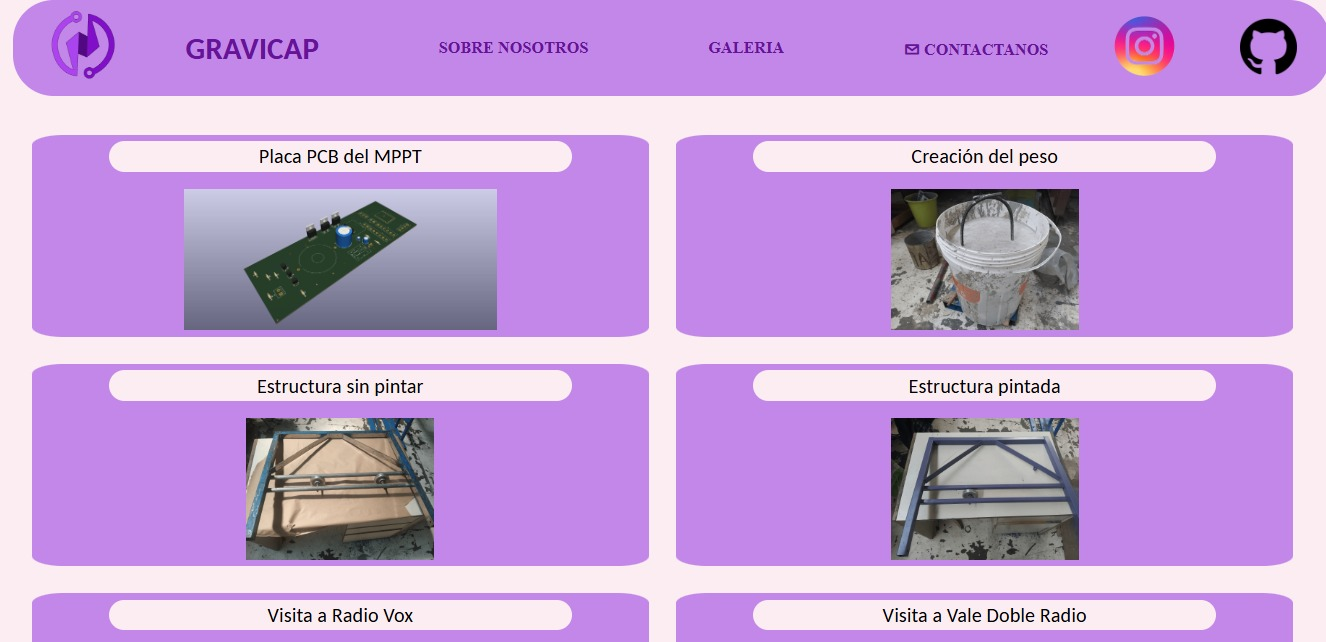
\includegraphics[width=\textwidth]{Imagenes/Página Web/Computadora/Galería.jpg}
                        \caption{Computadora}
                        \label{fig:pw4.1}
                    \end{subfigure}
                    \hfill
                    \begin{subfigure}{0.4\textwidth}
                        \centering
                        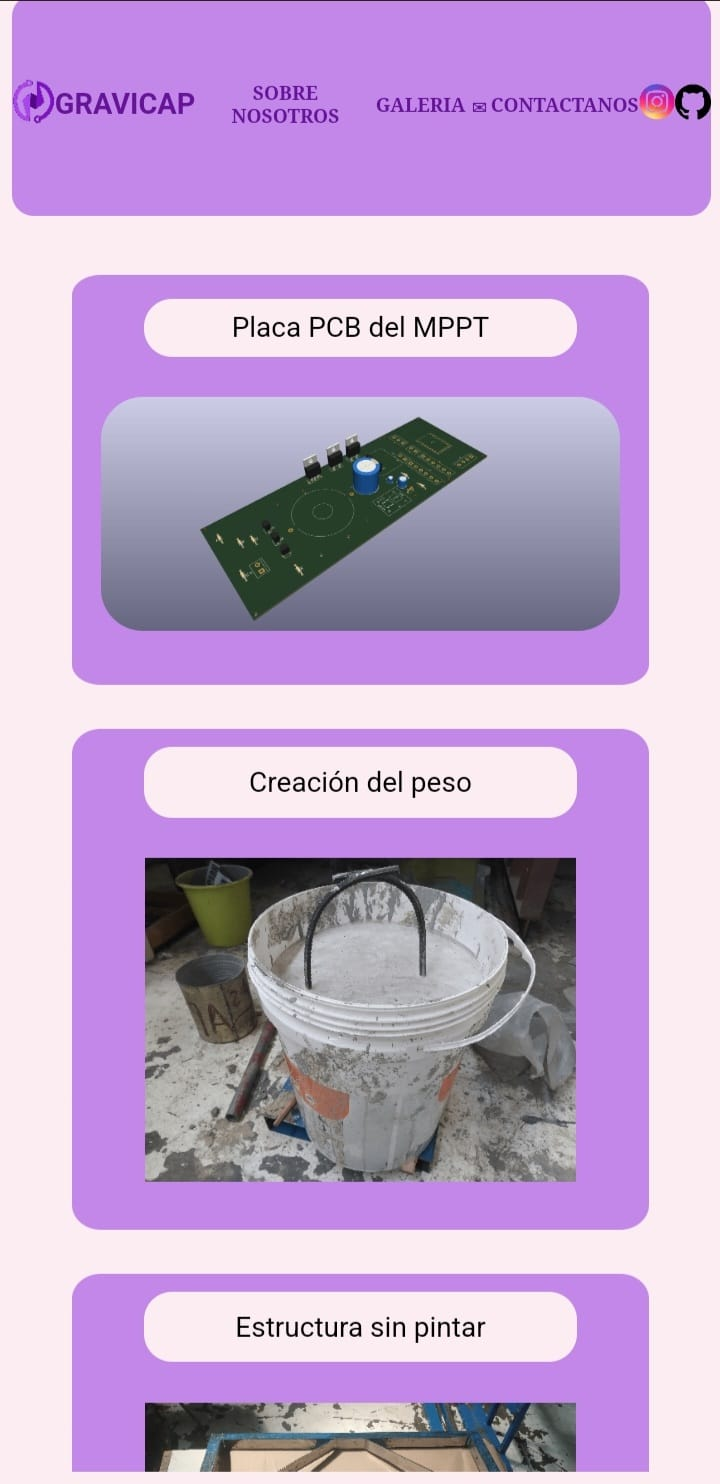
\includegraphics[width=0.5\textwidth]{Imagenes/Página Web/Celular/Galería.jpg}
                        \caption{Celular}
                        \label{fig:pw4.2}
                    \end{subfigure}
                    \hfill
                            
                    \caption{Componente de GaleríaView.vue}
                    \label{fig:pw4}
                    \end{figure}

                \subsubsection{ContactanosView.vue}
                    El subcomponente ContactanosView.vue incluye un formulario que permite a los usuarios enviarnos un mensaje directo a nuestra cuenta de Gmail del proyecto. El formulario solicita que el usuario ingrese su nombre, su correo electrónico y el mensaje que desea enviar. Una vez completado, se utiliza web3forms para procesar y enviar el mensaje, facilitando la comunicación directa entre los interesados y el equipo de \textcolor{dark_violet}{GraviCap}.\par

                    \begin{figure} [H]
                    \centering
                    \begin{subfigure}{0.5\textwidth}
                        \centering
                        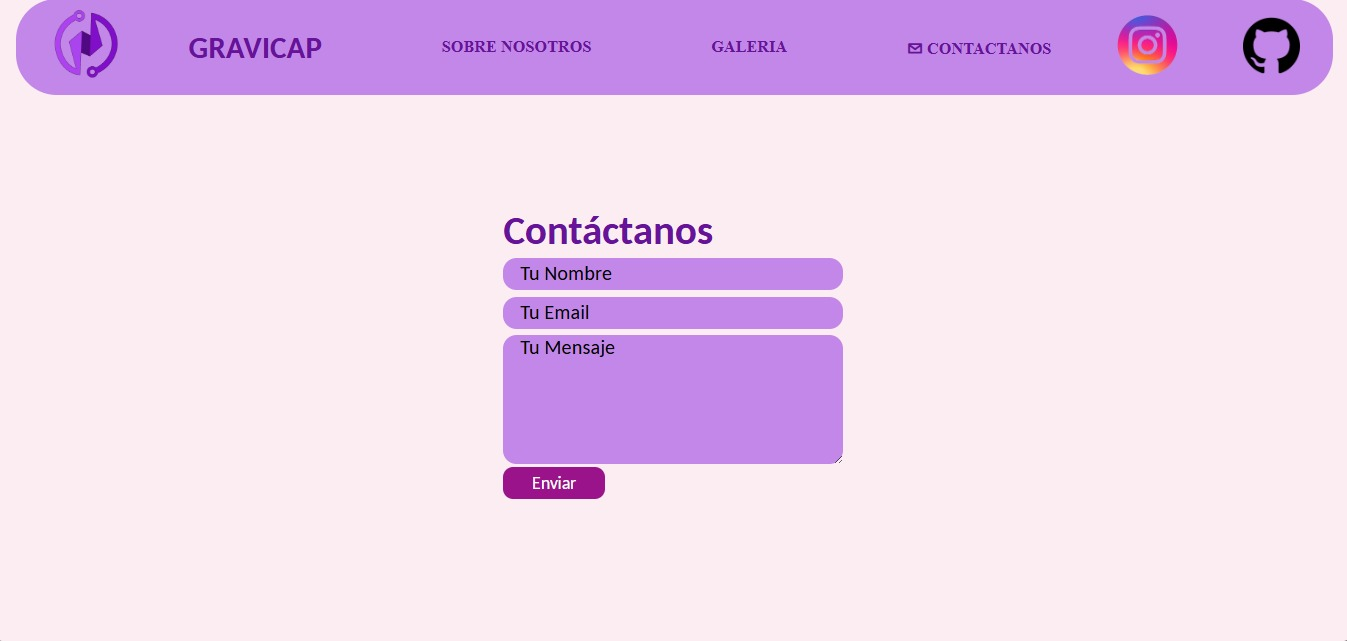
\includegraphics[width=\textwidth]{Imagenes/Página Web/Computadora/Contactos.jpg}
                        \caption{Computadora}
                        \label{fig:pw5.1}
                    \end{subfigure}
                    \begin{subfigure}{0.4\textwidth}
                        \centering
                        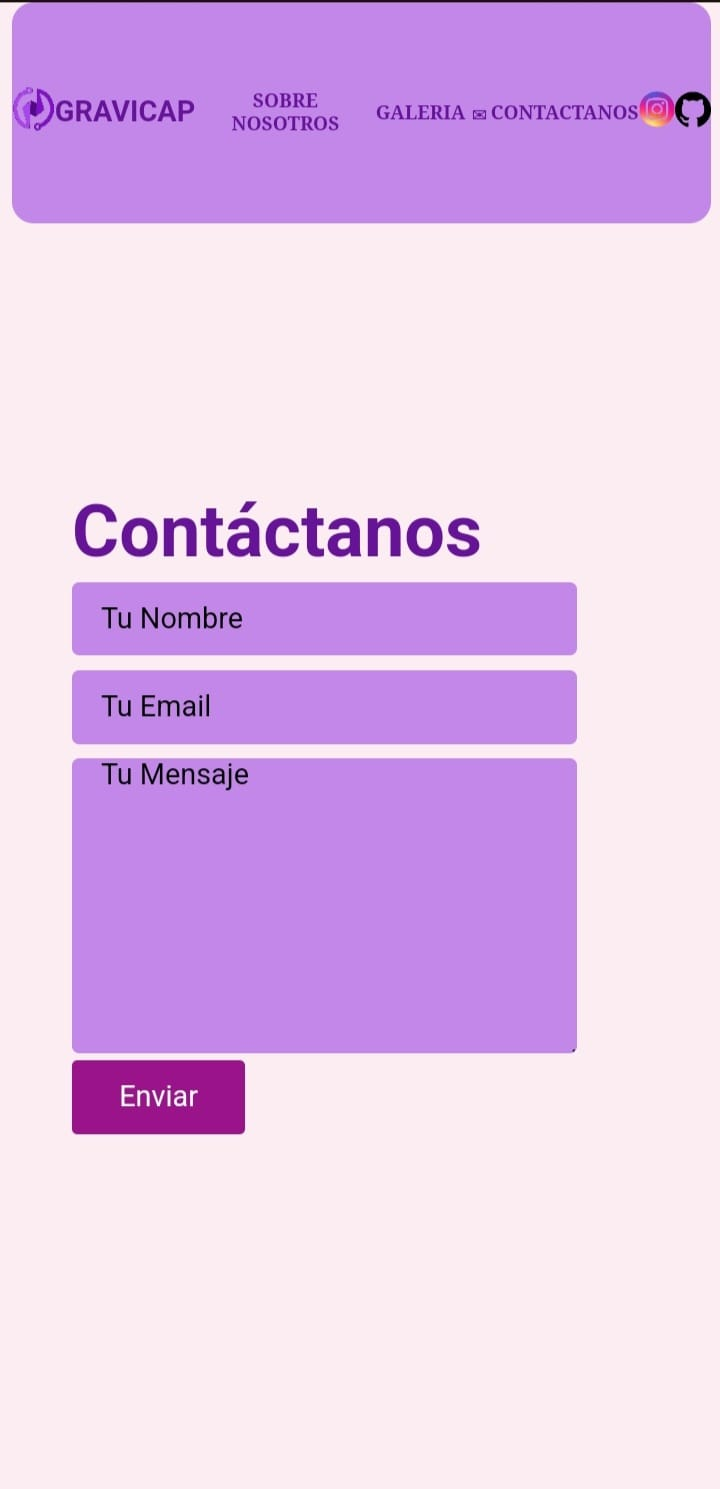
\includegraphics[width=0.5\textwidth]{Imagenes/Página Web/Celular/Contactos.jpg}
                        \caption{Celular}
                        \label{fig:pw5.2}
                    \end{subfigure}
                    \hfill
                            
                    \caption{Componente de ContactanosView.vue}
                    \label{fig:pw5}
                    \end{figure}
                    
    \section{Proceso}
        El desarrollo de la página web comenzó con la creación de los componentes principales en archivos separados de HTML y CSS, que definían tanto la estructura visual como la funcionalidad básica de cada parte de la página. El HTML se utilizó para definir la base de cada componente, mientras que el CSS permitió estilizar estos elementos y asegurarse de que fueran responsivos, es decir, que se ajustaran correctamente a diferentes tamaños de pantalla.\par
        Una vez diseñados estos componentes, se convirtieron en archivos .vue que incluyen tanto los estilos en CSS dentro de un bloque \texttt{<style scoped>} como la estructura HTML en un bloque \texttt{<template>}, permitiendo la integración en el framework Vue.js. Los componentes principales (HomeView.vue, ContactanosView.vue, GaleríaView.vue y NosotrosView.vue) fueron organizados en la carpeta views, mientras que el archivo App.vue se configuró para contener el \textit{header} y permitir la navegación entre las distintas secciones de la página.\par
        Finalmente, se creó un archivo index.js para manejar las rutas entre los diferentes componentes, facilitando la navegación entre las distintas secciones del sitio. El proyecto fue desplegado utilizando Vercel.app, una plataforma que permite alojar proyectos web fácilmente, y está disponible en el repositorio de GitHub del proyecto.\par